\section{Introduzione}


Lo studio delle proprietà cellulari e dello stato di vita della cellula è fondamentale nella ricerca. Diverse analisi mostrano come cellule con differenti stati vitali mostrano proprietà dielettriche diverse che possono dar luogo a segnali misurati differenti tra loro.

Si affronta la misurazione tramite citometro ad impedenza e l'analisi di un modello semplificato. Tale modello prevede un'equivalente circuitale e si presta per modellare il segnale di picco, con la cellula tra i due elettrodi.

Il modello si avvale anche della teoria delle miscele di Maxwell per omogeneizzare le proprietà dielettriche al fine di stimare un'unica permettività complessa e quindi l'impedenza risultate del sistema tramite la quale ricavare il segnale.

Nonostante la semplicità, rispetto altri approcci più completi quali la modellazione FEM, questo approccio permette di ottenere risultati molto veloci e utili alla distinzione tra diverse proprietà dielettriche di membrana.

Vengono quindi affrontate la modellazione e l'analisi di come variazioni delle proprietà dielettriche dei singoli costituenti si riflettono sul segnale modellato.

Tali proprietà tipicamente sono specchio dello stato di vita cellulare ed è possibile utilizzare questa modellazione per distinguere segnali provenienti da diverse famiglie cellulari quali cellule apoptodiche, cellule in salute o cellule necrotiche.

\section{Background}

\begin{figure*}[h!]
	\begin{subfigure}{0.5\linewidth}
			\centering
				\footnotesize{\def\svgwidth{0.95\linewidth}
				\input{citometro.pdf_tex}}
				\caption{}
	\end{subfigure}\hfill
	\begin{subfigure}{0.5\linewidth}
	\centering
	\footnotesize{\def\svgwidth{0.8\linewidth}
	\input{cell.pdf_tex}}
	\caption{}
\end{subfigure}\hfill
	\caption{Schema circuitale di misura nel citometro ad impedenza e tipico segnale (a); equivalente circuitale per cellula nel mezzo (b). Il segnale bipolare presenta il picco nel momento in cui la cellula passa tra le coppie parallele di elettrodi tale segnale può essere modellato, al variare della frequenza di misura, in uno schema circuitale equivalente. Nello sono trascurate eventuali impedenze parassite.}
	\label{fig:modellocircuitale}
\end{figure*}



La modellazione tramite equivalente circuitale porta in contro la teoria delle miscele di Maxwell (MMT) per modellare le proprietà dielettriche cellulari.

Tale modello permette di descrivere il segnale ottenuto in un citometro ad impedenza ad elettrodi paralleli nel momento in cui la cellula si trova tra una coppia di elettrodi. La presenza della cellula tra gli elettrodi, insieme alla perturbazione del campo elettrico, genera un segnale di corrente differenziale che risulta proporzionale al diametro per il tramite del fattore di Clausis-Mossotti.

Nel seguente report verrà considerata una versione semplificata del segnale, trascurando fattori aggiuntivi legati alle proprietà del circuito di misura, ovvero pari a:

\begin{equation}
	S=r^{3} f_{C M}
	\label{eq:signal}
\end{equation}

\subsection{Equivalenza circuitale}

Il circuito in \cref{fig:modellocircuitale} prevede l'applicazione di un potenziale agli elettrodi superiori e il campionamento del segnale dagli elettrodi inferiori, come corrente differenziale \cite{honradoSinglecellMicrofluidicImpedance2021}.

Osservando il percorso della corrente essa si troverà a passare per gli elettrodi e poi per il buffer conduttivo, eventualmente anche incontrando la cellula. Ognuno di questi materiali contribuirà con una sua impedenza.

Tali impedenze sono in serie e quindi il segnale misurato sarà:

\begin{equation}
	I_{\operatorname{d i f f}}=\frac{V_{\operatorname{a p p l}}}{Z_{\operatorname{m e d}}+2 Z_{d l}}-\frac{V_{\operatorname{a p p l}}}{Z_{\operatorname{m i x}}+2 Z_{d l}}
\end{equation}

Dove l'impedenza $Z_{\operatorname{m i x}}$ rappresenta l'insieme di cellula e buffer conduttivo e verrà descritta più avanti tramite MMT.

Inoltre, in questo segnale, riorganizzando i termini, compare una differenza di impedenza $\Delta Z=Z_{\operatorname{m i x}}-Z_{\operatorname{m e d}}$ pari proprio alla perturbazione indotta dalla cellula.  Tale termine inoltre risulta molto minore dell'impedenza del mezzo e questo ci permette di trascurare i termini quadratici e ottenere un segnale di corrente differenziale pari a:

\begin{equation}
	I_{\operatorname{d i f f}}\approx {V_{\operatorname{a p p l}}\over Z_{\operatorname{m e d}}^2} \frac{Z_{\operatorname{m i x}} -Z_{\operatorname{m e d}}}{\left(1+ 2{Z_{dl}\over Z_{\operatorname{m e d}} }\right)^2}
	\label{eq:idiff}
\end{equation}

L'impedenza di elettrodo è legata alla capacità superficiale $C_{dl}$ e alle dimensioni del volume del canale compreso tra le coppie. Risulta essere pari a:

\begin{equation}
	Z_{d l}=\frac{1}{j \omega C_{d l} w l}
\end{equation}

L'impedenza del mezzo viene espressa tramite la legge di Ohm, contestualizzandola in funzione del volume del canale:

\begin{equation}
	Z_{\operatorname{m e d}}=\frac{h}{\sigma^{*} l w k}={1\over \sigma^*}{1\over G}={1\over j\omega \varepsilon ^*}{1\over G}
\end{equation}

Portando in conto anche effetti di distorsione del campo elettrico tramite un coefficiente geometrico $G$. 

In generale, la permittività complessa è esprimibile come:

\begin{equation}
	\varepsilon^{*}=\varepsilon+\frac{\sigma}{j \omega}
\end{equation}

Tali considerazioni sono analoghe per l'impedenza del mix dove però la $\varepsilon^*_{\operatorname{m i x}}$ va stimata tramite la teoria delle miscele di Maxwell. 

\subsection{Maxwell's Mixtures theory}
\begin{figure*}[t!]
	\centering
	\footnotesize{\def\svgwidth{0.95\linewidth}
		\input{homogenization.pdf_tex}}
	\caption{Omogenizzazione secondo il modello double shell. Si affronta una doppia omogeneizzazione, prima per il nucleo passando ad un materiale omogeneo (nuc). Tale materiale viene poi omogenizzato con il citoplasma (omogeneizzazione rispetto al mezzo in cui è immersa una particella) e infine si omogenizza l'interno della cellula con la membrana. Quest'ultimo passaggio corrisponde all'omogeneizzazione single shell.}
	\label{fig:screenshot001}
\end{figure*}

\begin{table*}[t!]
	\centering
	\small{
		\begin{tabular}{|l|c|c|c|c|}
			\hline
			Flag & $\mathtt{radius}$ [m] & $\mathtt{sgm\_mem}$ [S/m] &$\mathtt{ sgm\_int}$ [S/m] & $\mathtt{eps\_int }$ \\
			\hline
			$\mathtt{bead}$ & 3e-6 & 1e10 & 2.7e-3 & 2.5$\cdot \varepsilon_0$ \\
			\hline
			$\mathtt{viable}$ & 9e-6 & 0 & 0.6 & 60$\cdot \varepsilon_0$ \\
			\hline
			$\mathtt{necrotic}$ & 9e-6 & 1e-3 & 0.6 & 60$\cdot \varepsilon_0$ \\
			\hline
			$\mathtt{apoptotic \:intact}$ & 3e-6 & 0 & 0.6 & 60$\cdot \varepsilon_0$\\
			\hline
			$\mathtt{apoptotic\: permeable}$ & 3e-6 & 1e-3 & 0.6 & 60$\cdot \varepsilon_0$ \\
			\hline
	\end{tabular}}
	\caption{Parametri per il modello single shell. Differenti stati biologicim ostrano differenti proprietà dielettriche.}
	\label{tab:data}
\end{table*}


La teoria delle miscele di Maxwell permette di descrivere la permettività complessa di mezzo e cellula in funzione delle loro proprietà \cite{hanai_method_1975}.

In particolare, si può esprimere la permettività in funzione del fattore di Clausius-Mossotti come:

\begin{equation}
	\varepsilon_{\operatorname{mix}}^{*}=\varepsilon_{\operatorname{m e d}}^{*} \frac{1+2 \varphi f_{C M}}{1-\varphi f_{C M}}
	\label{eq:permett}
\end{equation}

A sua volta questo fattore si esprime in funzione delle proprietà della cellula:

\begin{equation}
	f_{C M}=\frac{\varepsilon_{\operatorname{c e l l}}^{*}-\varepsilon_{\operatorname{m e d}}^{*}}{\varepsilon_{\operatorname{c e l l}}^{*}+2 \varepsilon_{\operatorname{m e d}}^{*}}
\end{equation}

Mettendo insieme quanto descritto si ottiene l'espressione per la corrente differenziale in \cref{eq:idiff}, in funzione del fattore di Clausius-Mossotti:

\begin{equation}
	I_{d i f f} \approx-\frac{V_{\operatorname{a p p l}}}{Z_{\operatorname{m e d}}} \frac{1}{\left[1+\frac{2 Z_{d l}}{Z_{\operatorname{m e d}}}\right]^{2}} 3 \varphi f_{CM}
\end{equation}

Dove $\varphi$ è la volume fraction che porta in conto il volume della cellula come:

\begin{equation}
	\varphi=\frac{V_{\text {cell }}}{V_{\text {misura }}}=\frac{\frac{4 \pi r^{3}}{3}}{l w h K}
\end{equation}

E il segnale misurato, trascurando i contributi dispersivi legati agli elettrodi, risulta proporzionale a $r^3$ (tramite la volume fraction) e al fattore di Clausius-Mossotti.





\begin{figure*}[t!]
	\begin{subfigure}{0.5\linewidth}
		\centering
		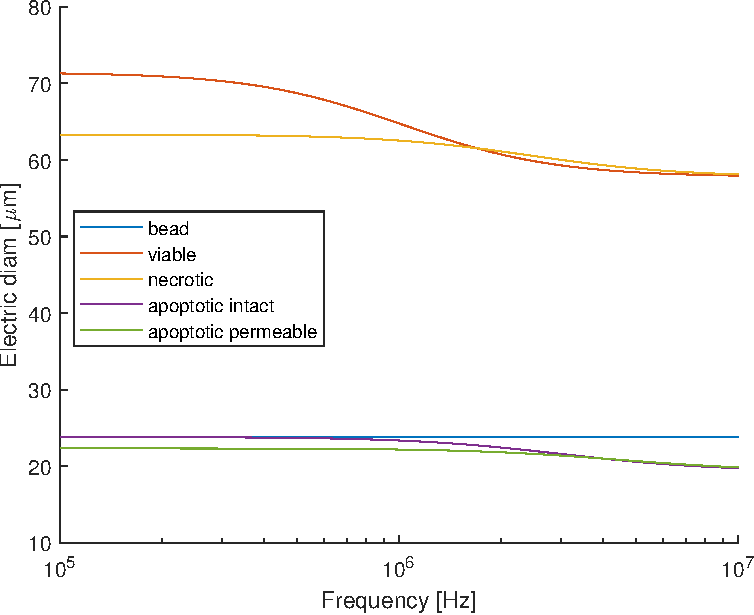
\includegraphics[width=0.95\linewidth]{../code/figs/diam}
		\caption{}
		\label{fig:diam}
	\end{subfigure}\hfill
	\begin{subfigure}{0.5\linewidth}
		\centering
		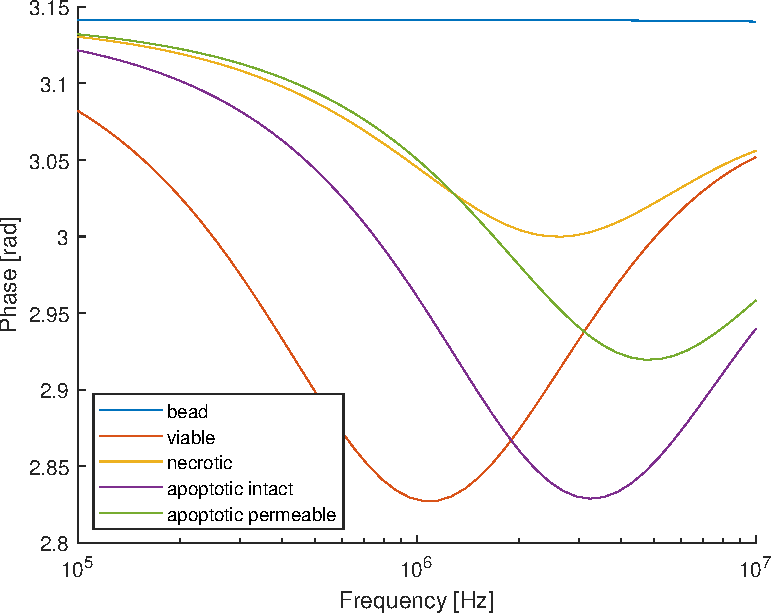
\includegraphics[width=0.95\linewidth]{../code/figs/phase}
		\caption{}
		\label{fig:phase}
	\end{subfigure}
	\caption{Andamento del segnale ottenuto dal modello single shell al variare delle proprietà cellulari, rappresentato come diametro elettrico, proporzionale alla radice cubica del modulo (a) e fase (b)}
	\label{fig:risultati}
\end{figure*}

\begin{figure}[b!]
	\centering
	\footnotesize{\def\svgwidth{0.95\linewidth}
	\input{str.pdf_tex}}
	\caption{Rappresentazione della gerarchica di struttura utilizzata per portare in conto le proprietà degli elementi della cellula}
	\label{fig:structure}
\end{figure}


\subsection{Shell model}

Avendo visto come portare in conto le proprietà miste di cellula e mezzo non rimane che analizzare come omogeneizzare le proprietà della singola cellula. 
Le cellule vengono omogenizzate ad un unico materiale avente proprietà $\varepsilon^*_{\operatorname{cell}}$ e tale da portare in conto sia le proprietà della parte interna che della membrana cellulare.

Per cellule prive di nucleo, come i globuli rossi, è possibile utilizzare un modello \textbf{single shell}, basato quindi su una membrana esterna sottile ed una zona interna le cui proprietà vengono omogeneizzate come:

\begin{equation}
	\varepsilon_{c e l l}^{*} \approx \varepsilon_{i n t}^{*} \frac{\chi}{1+\chi}
	\label{eq:shell}
\end{equation}

Dove:

\begin{equation}
	\chi=\frac{\varepsilon_{m e m}^{*} / d_{m e m}}{\varepsilon_{i n t}^{*} / r}
\end{equation}

Per cellule più grandi e complesse è necessario considerare un modello più accurato come il \textbf{double shell} dove vengono considerate quattro differenti zone. Si considera una zona interna, corrispondente al nucleo, ($\operatorname{np}$) e la sua membrana $\operatorname{ne}$. A queste si aggiunge il citoplasma $\operatorname{cyt}$ e la membrana cellulare $\operatorname{mem}$. 

In particolare, si effettuano delle omogenizzazioni in sequenza partendo dalla zona centrale. 

Applicando una relazione analoga a \cref{eq:shell} si arriva a stimare le proprietà complessive del nucleo ($\operatorname{nuc}$). Successivamente queste possono essere unite proprio tramite la MMT descrivendo così l'interno cellulare ($\operatorname{int}$). Infine, si ripete l'omogenizzazione (\cref{eq:shell}) tra la zona interna e la membrana ottenendo così una permittività complessa per l'intera cellula. 


\section{Risultati}


\begin{figure*}[t!]
	\centering
	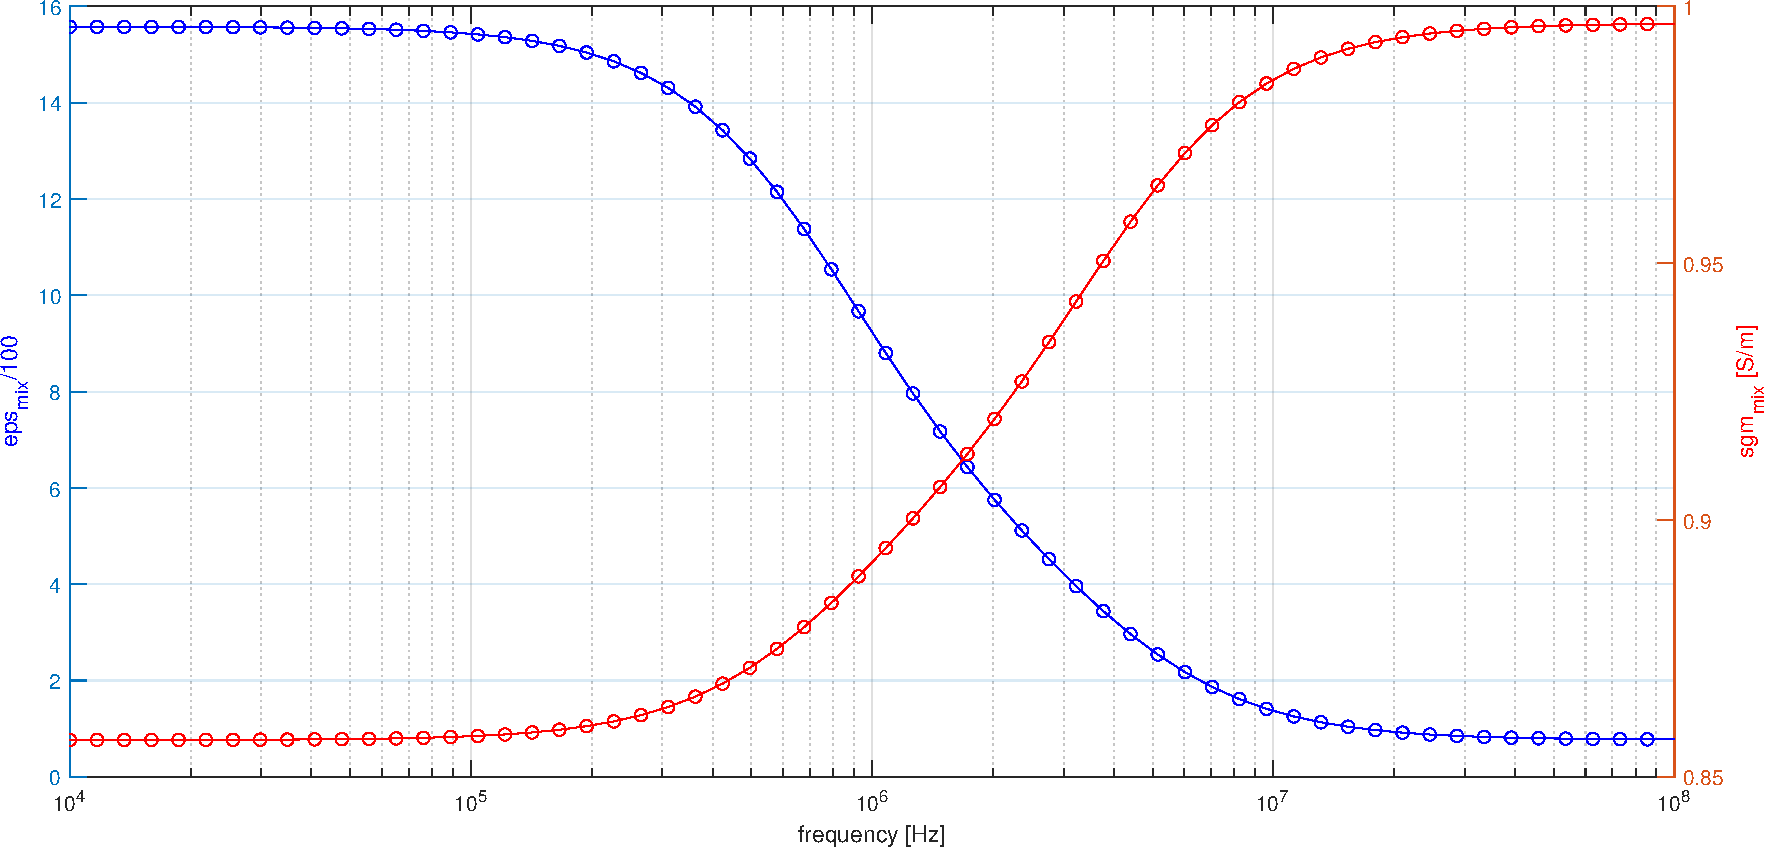
\includegraphics[width=0.95\linewidth]{../code/figs/epstilde_mix_plot}
	\caption{Andamento della permettività complessa (parte reale e immaginaria) per il modello double shell al variare della frequenza.}
	\label{fig:epstildemixplot}
\end{figure*}



Vengono quindi applicati questi modelli per stimare segnali di citometria ad impedenza di diverse famiglie cellulari in stato vitale, necrotico e apoptotico \cite{de_ninno_high-throughput_2020}.
I parametri utilizzati, da \citeauthor{de_ninno_high-throughput_2020}, sono riportato in \cref{tab:data}.

Al fine di rappresentare la fisica del problema sono state utilizzate, all'interno di Matlab, le variabili di classe struttura. Tali variabili permettono l'aggiunta di alcuni campi e quindi si è utilizzata la sequenza dei campi per rappresentare le proprietà possedute dalla struttura madre. Ad esempio, la permettività della membrana cellulare sarà il campo $\mathtt{eps}$ della struttura $\mathtt{mem}$ a sua volta figlia di $\mathtt{cell}$. 

Uno schema grafico è presente, per la formulazione double shell, in \cref{fig:structure}, e un esempio in appendice.

Tale struttura, oltre ad essere rappresentativa dell'elemento fisico che possiede tale proprietà, permette di iterare alcune procedure andando a prendere i singoli campi di diverse strutture e di realizzare un codice modulare e facilmente estensibile ed aggiornabile.

Il codice prevede una routine principale \texttt{main.m} e diverse routine ausiliarie.

I dati vengono caricati tramite la routine \texttt{data(flag)} passando la flag indicata in \cref{tab:data} per ottenere i relativi parametri e le strutture $\mathtt{cell}$ e $\mathtt{med}$.

La routine principale itera sulle differenti flag per poi ottenere il segnale in \cref{fig:risultati}. Per ogni iterazione, dopo aver richiamato le proprietà materiali, queste vengono passate alla routine $\mathtt{equivalenteCircuitModel.m}$ che si occupa di modellare il circuito equivalente e restituire il segnale come in \cref{eq:signal} e la permettività complessa omogeneizzata (\cref{eq:permett}, tramite $\mathtt{fcm\_mix()}$).

Per farlo necessita del calcolo delle proprietà omogeneizzate della cellula e del fattore di Clausius-Mossotti. Quest'ultimo viene calcolato tramite una routine corrispondente. 

L'omogeneizzazione delle proprietà cellulari viene effettuata tramite la routine \texttt{MMT.m} che viene suddivisa, tramite il campo $\mathtt{cell.shell}$ nell'implmentazione single shell o double shell.  

Tale routine, oltre a calcolare le relative quantità complesse per il tramite della routine \texttt{epstile.m} calcola l'omogeneizzazione per il tramite della subroutine \texttt{mixture.m} che applica l'\cref{eq:shell}.

Dal segnale ottenuto è possibile ricavare il diametro elettrico come la radice cubica del modulo e i risultati sono presenti in \cref{fig:diam}, insieme alla fase del segnale in \cref{fig:phase}.

Dall'analisi dei grafici è possibile identificare differenti peculiarità a seconda delle famiglie che si vogliono distinguere. Effettuando misurazioni a differenti frequenze sarà possibile distinguere tra diversi stati vitali nella popolazione analizzata.




\subsection{Modello double-shell}

Per l'implementazione double-shell è sufficiente inserire i campi richiesti per le proprietà cellulari. I parametri utilizzati, noti in letteratura \cite{irimajiri_dielectric_1979}, sono presenti in \cref{tab:double_shell}.

Inseriti i parametri nelle proprietà della struttura $\mathtt{cell}$, la routine \texttt{MMT()} si occupa di fare la doppia omogeneizzazione e restituirne i valori della $\varepsilon_{\operatorname{mix}}^*$. 

Tali valori sono graficati per il tramite della routine \texttt{mix\_plot()} che si occupa di normalizzare i valori e restituire i grafici di $\varepsilon$ e $\sigma$ presente in \cref{fig:epstildemixplot}.









\subsubsection{Influenza delle variazioni dei singoli parametri}



Inoltre, si analizza l'influenza delle perturbazioni sugli otto parametri descrittivi del modello double shell. Le variazioni vengono effettuate secondo \citeauthor{irimajiri_dielectric_1979} \cite{irimajiri_dielectric_1979}.

Vengono quindi caricati i dati delle perturbazioni tramite la struttura $\mathtt{perturbation\_values.data}$ e viene iterata la stessa procedura sugli otto parametri. Il risultato è presente in \cref{fig:perturbazioni}. 

Un esempio della procedura di iterazione è presente in appendice.

\begin{table}[t!]
	\centering
	\small{
		\begin{tabular}{|c|c|c|c|c|}
			\hline
			$\mathtt{cell}$ & $\mathtt{.np}$  & $\mathtt{.ne}$  &$\mathtt{.cyt}$ & $\mathtt{.mem}$ \\
			\hline
			$\mathtt{.eps}$ $\cdot \varepsilon_0$ &77  & 40 & 1e10 &77  \\
			\hline
			$\mathtt{.sgm}$ [S/m]& 1 & 4e-4 & 1 & 8e-8$\cdot \varepsilon_0$ \\
			\hline
	\end{tabular}}
	\caption{Parametri utilizzati per i campi della struttura $\mathtt{cell}$ nel modello double shell.}
	\label{tab:double_shell}
\end{table}

\begin{figure*}[t!]
	\begin{subfigure}{0.5\linewidth}
		\centering
	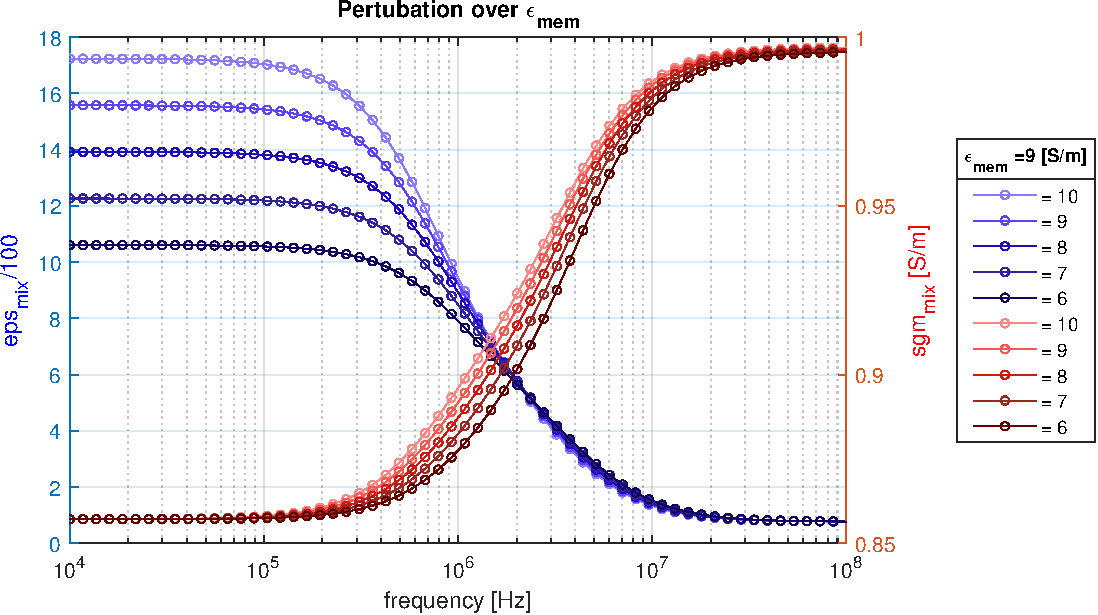
\includegraphics[width=0.95\linewidth]{../code/figs/eps_mem_pert}
		\caption{}
		\label{fig:epsmempert}
	\end{subfigure}\hfill
	\begin{subfigure}{0.5\linewidth}
		\centering
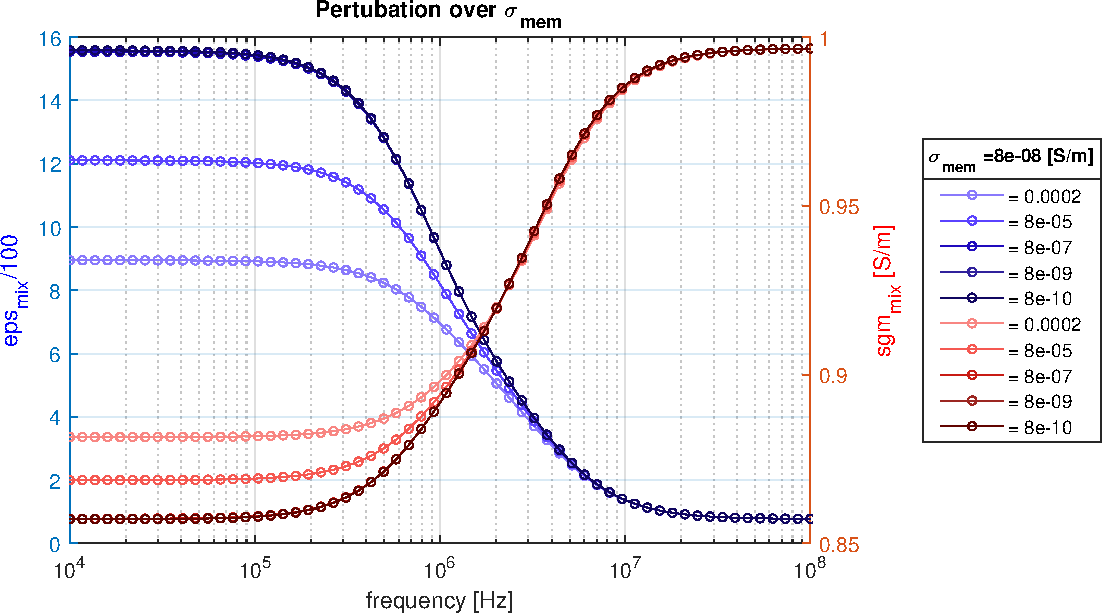
\includegraphics[width=0.95\linewidth]{../code/figs/sgm_mem_pert}
\caption{}
\label{fig:sgmmempert}
	\end{subfigure}\vspace{0.6cm}
	\begin{subfigure}{0.5\linewidth}
	\centering
	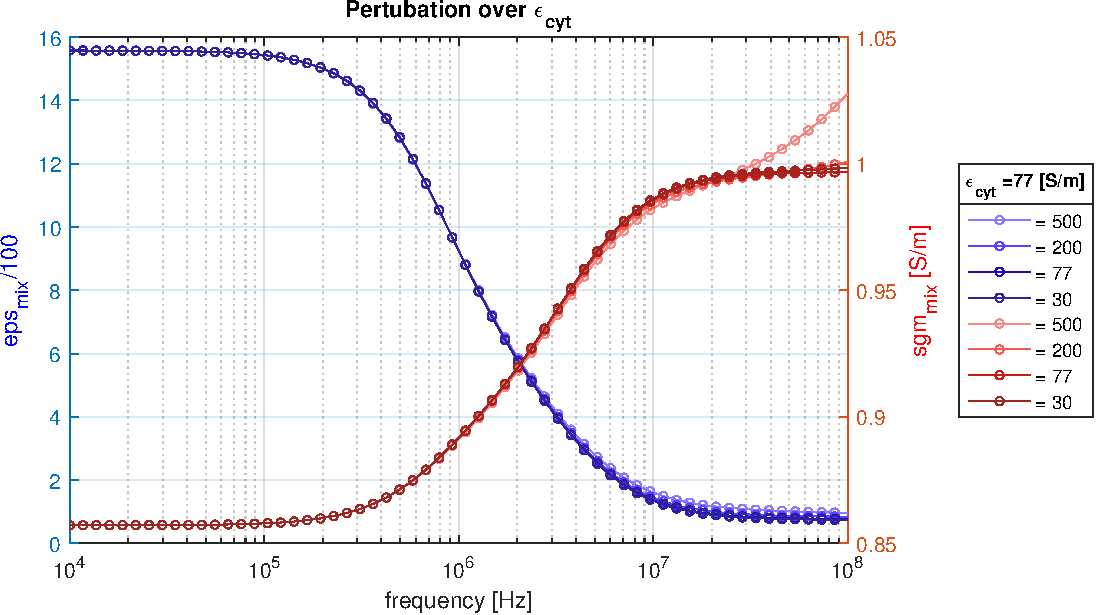
\includegraphics[width=0.95\linewidth]{../code/figs/eps_cyt_pert}
	\caption{}
	\label{fig:epscytpert}
\end{subfigure}\hfill
\begin{subfigure}{0.5\linewidth}
	\centering
	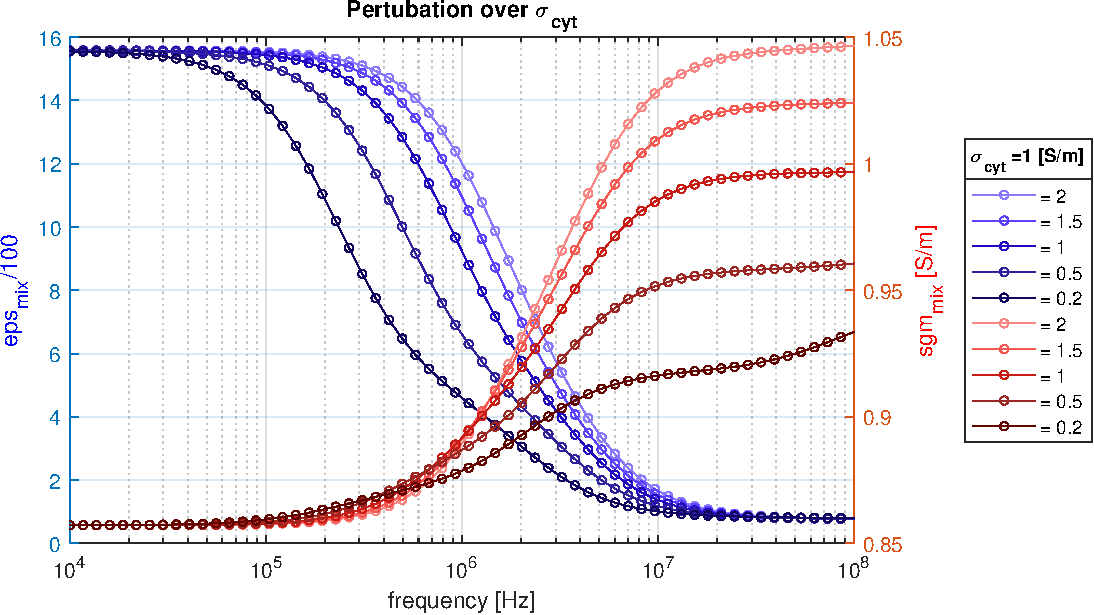
\includegraphics[width=0.95\linewidth]{../code/figs/sgm_cyt_pert}
	\caption{}
	\label{fig:sgmcytpert}
\end{subfigure}\vspace{0.6cm}
	\begin{subfigure}{0.5\linewidth}
	\centering
	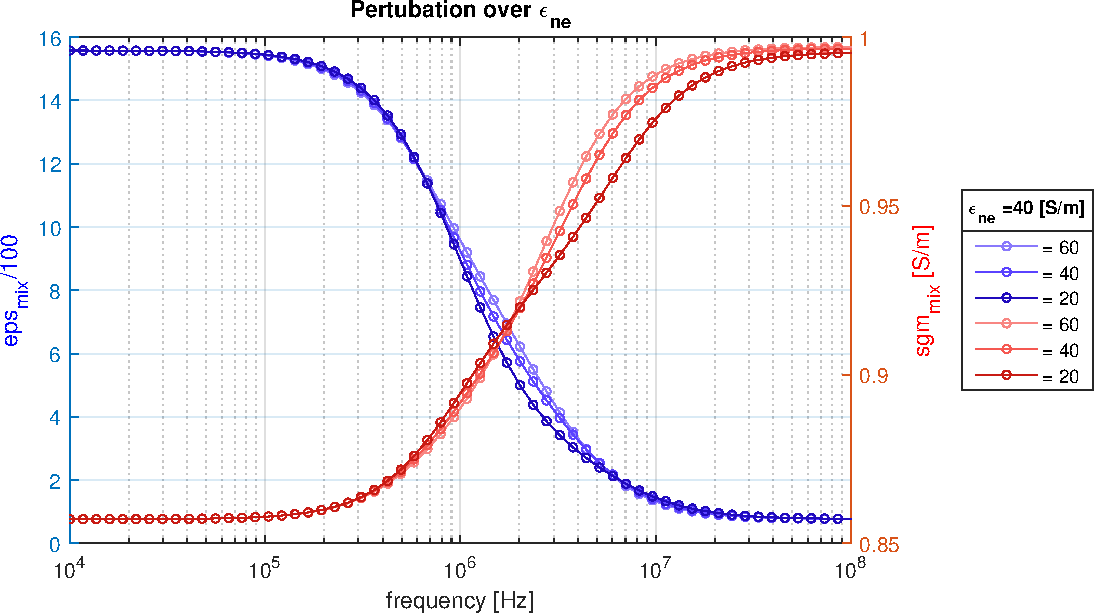
\includegraphics[width=0.95\linewidth]{../code/figs/eps_ne_pert}
	\caption{}
	\label{fig:epsnepert}
\end{subfigure}\hfill
\begin{subfigure}{0.5\linewidth}
	\centering
	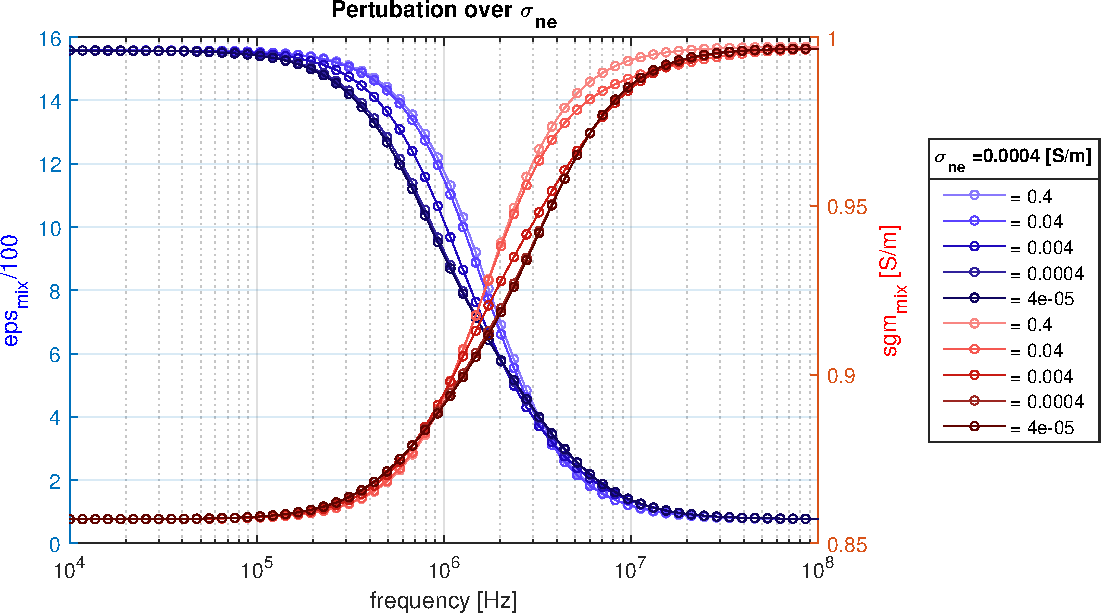
\includegraphics[width=0.95\linewidth]{../code/figs/sgm_ne_pert}
	\caption{}
	\label{fig:sgmnepert}
\end{subfigure}\vspace{0.6cm}
	\begin{subfigure}{0.5\linewidth}
	\centering
	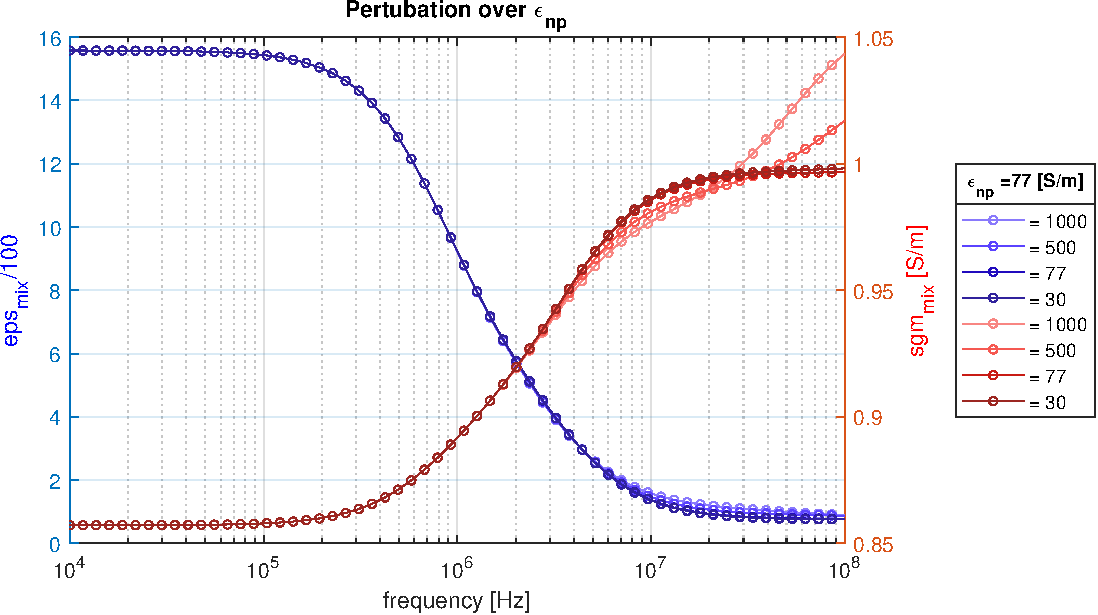
\includegraphics[width=0.95\linewidth]{../code/figs/eps_np_pert}
	\caption{}
	\label{fig:epsnppert}
\end{subfigure}\hfill
\begin{subfigure}{0.5\linewidth}
	\centering
	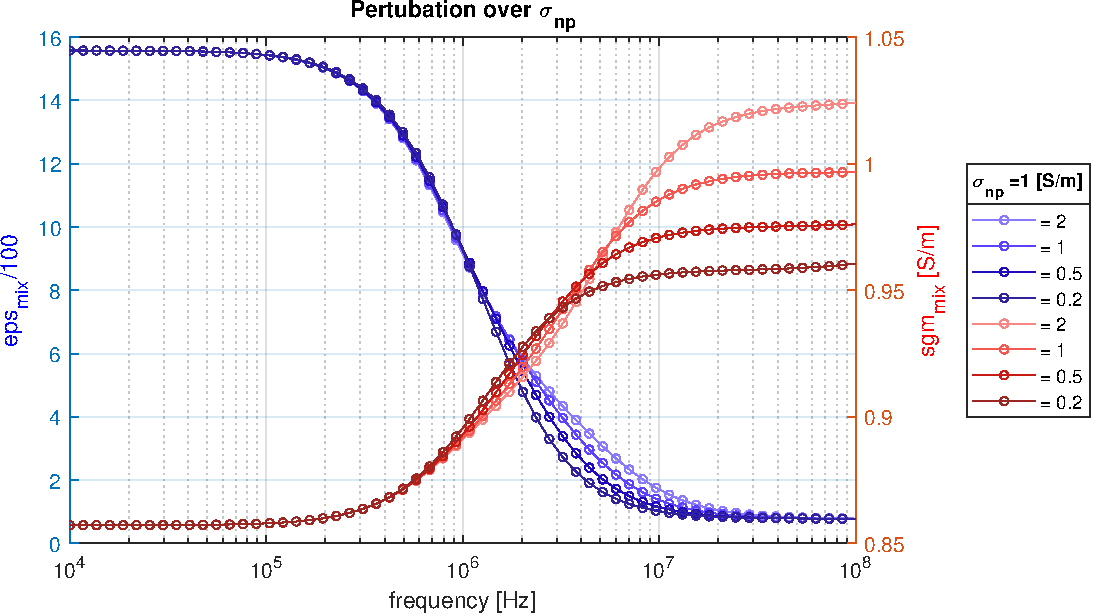
\includegraphics[width=0.95\linewidth]{../code/figs/sgm_np_pert}
	\caption{}
	\label{fig:sgmnppert}
\end{subfigure}\hfill
	\caption{Variazione delle proprietà materiali per gli 8 parametri del modello double shell. I grafici rappresentano la variazione di $\varepsilon$ (a destra) e $\sigma$ (a sinistra) per la membrana cellulare (a,b), citoplasma (c,d), membrana nucleare (e,f) e nucleo (g,h). Nella legenda è presenta il valore originale, nel riquadro, e i rispetti valori di test.}
	\label{fig:perturbazioni}
\end{figure*}

Dai grafici è possibile vedere come il comportamento a bassa frequenza viene influenzato principalmente dalla variazione degli strati esterni con predominanza per le proprietà di membrana.

Ad alta frequenza la permettività viene influenzata poco e principalmente variando le proprietà di citoplasma e nucleo mentre la conduttività risente molto delle variazioni delle proprietà di citoplasma e nucelo.

Nella banda centrale la pendenza delle curve risente notevolmente della variazione di $\sigma_{\operatorname{cyt}}$.

In generale, le variazioni delle proprietà di conduttività hanno effetti maggiori sulla permettività complessa omogeneizzata.
	
	
\section{Conclusioni}


Tali evidenti variazioni delle proprietà omogeneizzate possono essere utilizzate per estrarre informazioni dai segnali di citometria al fine di analizzare lo stato di vita cellulare.

Differenti proprietà misurate forniscono segnali diversi ed è possibile utilizzare tale teoria per risalire dal segnale alla differenziazione tra diversi stati cellulari. 

Tramite l'analisi del modello a circuito equivalente con la teoria delle miscele di Maxwell è possibile capire a quale frequenza effettuare le misurazioni a seconda delle popolazioni cellulari che si vuole misurare. 


\raggedbottom


\raggedbottom
\pagebreak
\section*{Disponiblità dei dati}

Il materiale è disponibile alla repository online del progetto: \url{https://github.com/mastroalex/ecm-mmt}.

\printbibliography[title=Riferimenti]
%\section*{References}

\clearpage
\onecolumn
\section*{Appendice}

\subsection*{Caricamento dei dati all'interno della struttura}

A seguire uno snippet estratto dalla procedure \texttt{data.m} all'interno di uno switch-case sulla variabile $\mathtt{flag}$. Tale sezione di codice permette di caricare le strutture $\mathtt{cell}$ e $\mathtt{med}$ con i loro campi contenenti le proprietà dielettriche e geometriche, insieme alla flag \texttt{double} che permetterà, alle relative subroutine, di effettuare l'omogeneizzazione di tipo double shell.

\begin{figure}[h!]
	\begin{lstlisting}[language=matlab]
	case 'double'
		cell.shell='double';
		mem.thickness=80*1e-10; %[m]
		cell.radius=6.5*1e-6; %[m]
		int.radius=cell.radius;
		mem.sgm=8e-7*1e-1; %[S/m]
		mem.eps= 9*eps0; 
		int.sgm=0.6; 	int.eps=60*eps0;
		cell.int=int;	cell.mem=mem;
		cell.np.radius=4.67*1e-6;
		cell.ne.thickness=400*1e-10;
		cell.np.sgm=10*1e-1; 	cell.np.eps=77*eps0;
		cell.ne.sgm=4e-3*1e-1;	cell.ne.eps=40*eps0;
		cell.cyt.sgm=10*1e-1;	cell.cyt.eps=77*eps0;
		med.sgm= 1;	med.eps= 77*eps0;
		cell.volfrac=0.1; 	cell.nuc.volfrac=(cell.np.radius/cell.radius)^3;
	\end{lstlisting}
\end{figure}

\subsection*{Perturbazione}

Esempio di iterazione per la perturbazione della permettività della membrana cellulare. Viene riportato lo snippet della variazione di $\varepsilon_{\operatorname{m e m}}$. 

Una sequenza analoga viene utilizzata anche sugli altri 7 parametri analizzati.

\begin{figure}[h!]
	\begin{lstlisting}[language=matlab]
	% load pertubation values 
	pert=perturbation_values.eps.mem;
	% string for reference
	perturbation='{\epsilon}_{mem}'; 
	real_value=cell.mem.eps/eps0;
	% create figure and plot
	eps_mem_pert=figure();
	cell_pert=cell;
	for i=1:length(pert)
		% change perturbation properties
		cell_pert.mem.eps=pert(i);
		[~,~,cell_pert,epstile_mix_pert]=equivalentCircuitModel(med,cell_pert,frequency_span);
		mix_plot(eps_mem_pert,epstile_mix_pert,frequency_span,omega,{colorType1{i},colorType2{i}})
		clear epstile_mix_pert
	end
	% resize figs
	eps_mem_pert.Position = [100 100 800 400];
	lg=legend(strcat('='," ",string([pert/eps0,pert/eps0])),'Location','eastoutside');
	lg.Title.String=strcat(perturbation,' = ',num2str(real_value),' [S/m]');
	title(strcat('Pertubation over'," ",perturbation))
	\end{lstlisting}
\end{figure}